% exva_rand - ExVA on lego_random_exr (u4108)
% excol_coloc - ExCol on lego_coloc_exr (u4105)
\begingroup
\begin{figure}[!htb]
    % \setArraystrech{1.5}
    \centering
    \setlength\tabcolsep{2pt}
    \begin{tabular*}{\textwidth}{ c c c c c }
        \multicolumn{5}{c}{\textit{ExVA} trained on \textbf{arbitrary} light dataset} \\
          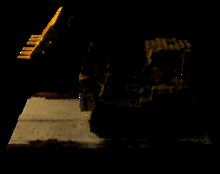
\includegraphics[width=0.19\textwidth]{figures/results/arb_set/dynamic_light/exva_rand_vc0_ld-90.png}
        & 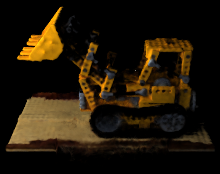
\includegraphics[width=0.19\textwidth]{figures/results/arb_set/dynamic_light/exva_rand_vc0_ld-60.png}
        & 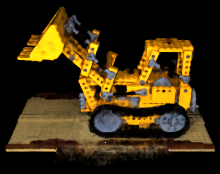
\includegraphics[width=0.19\textwidth]{figures/results/arb_set/dynamic_light/exva_rand_vc0_ld0.png}
        & 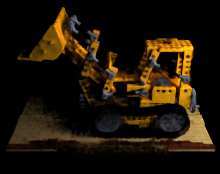
\includegraphics[width=0.19\textwidth]{figures/results/arb_set/dynamic_light/exva_rand_vc0_ld60.png} 
        & 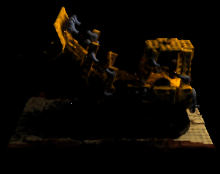
\includegraphics[width=0.19\textwidth]{figures/results/arb_set/dynamic_light/exva_rand_vc0_ld90.png} \\
        
        \multicolumn{5}{c}{\textit{ExCol} trained on \textbf{colocated} light dataset} \\
          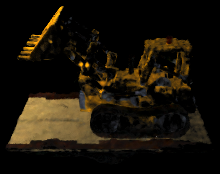
\includegraphics[width=0.19\textwidth]{figures/results/arb_set/dynamic_light/excol_col_vc0_ld-90.png}
        & 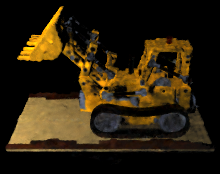
\includegraphics[width=0.19\textwidth]{figures/results/arb_set/dynamic_light/excol_col_vc0_ld-60.png}
        & 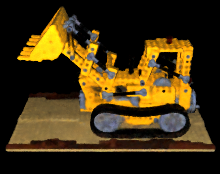
\includegraphics[width=0.19\textwidth]{figures/results/arb_set/dynamic_light/excol_col_vc0_ld0.png}
        & 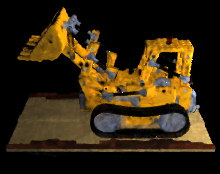
\includegraphics[width=0.19\textwidth]{figures/results/arb_set/dynamic_light/excol_col_vc0_ld60.png} 
        & 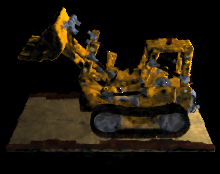
\includegraphics[width=0.19\textwidth]{figures/results/arb_set/dynamic_light/excol_col_vc0_ld90.png} \\

        \multicolumn{5}{c}{\textit{ImNF} trained on \textbf{colocated} light dataset} \\
          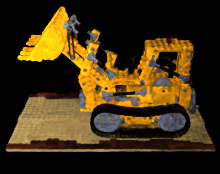
\includegraphics[width=0.19\textwidth]{figures/results/arb_set/dynamic_light/imnf_coloc_vc0_ld-90.png}
        & 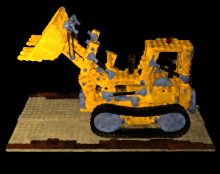
\includegraphics[width=0.19\textwidth]{figures/results/arb_set/dynamic_light/imnf_coloc_vc0_ld-60.png}
        & 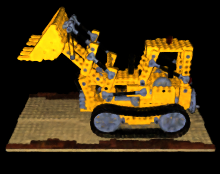
\includegraphics[width=0.19\textwidth]{figures/results/arb_set/dynamic_light/imnf_coloc_vc0_ld0.png}
        & 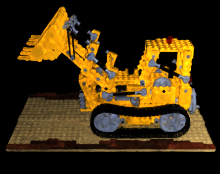
\includegraphics[width=0.19\textwidth]{figures/results/arb_set/dynamic_light/imnf_coloc_vc0_ld60.png} 
        & 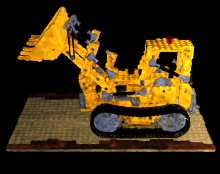
\includegraphics[width=0.19\textwidth]{figures/results/arb_set/dynamic_light/imnf_coloc_vc0_ld90.png} \\

        \multicolumn{5}{c}{\textit{ImNF} trained on \textbf{arbitrary} light dataset} \\
          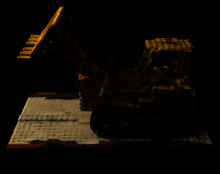
\includegraphics[width=0.19\textwidth]{figures/results/arb_set/dynamic_light/imnf_rand_vc0_ld-90.png}
        & 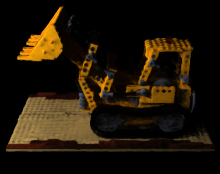
\includegraphics[width=0.19\textwidth]{figures/results/arb_set/dynamic_light/imnf_rand_vc0_ld-60.png}
        & 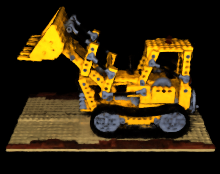
\includegraphics[width=0.19\textwidth]{figures/results/arb_set/dynamic_light/imnf_rand_vc0_ld0.png}
        & 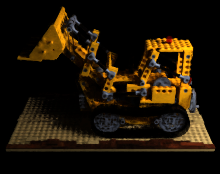
\includegraphics[width=0.19\textwidth]{figures/results/arb_set/dynamic_light/imnf_rand_vc0_ld60.png} 
        & 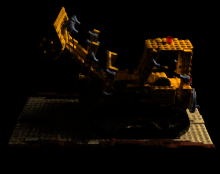
\includegraphics[width=0.19\textwidth]{figures/results/arb_set/dynamic_light/imnf_rand_vc0_ld90.png} \\
        
        \multicolumn{5}{c}{Target images} \\
          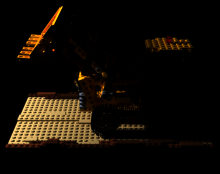
\includegraphics[width=0.19\textwidth]{figures/results/arb_set/dynamic_light/targ_vc0_ld-90.png}
        & 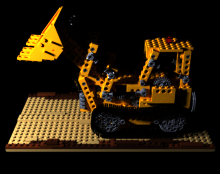
\includegraphics[width=0.19\textwidth]{figures/results/arb_set/dynamic_light/targ_vc0_ld-60.png}
        & 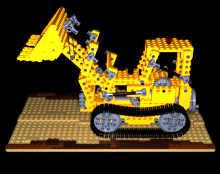
\includegraphics[width=0.19\textwidth]{figures/results/arb_set/dynamic_light/targ_vc0_ld0.png}
        & 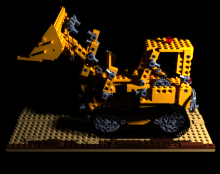
\includegraphics[width=0.19\textwidth]{figures/results/arb_set/dynamic_light/targ_vc0_ld60.png} 
        & 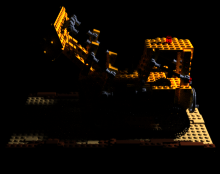
\includegraphics[width=0.19\textwidth]{figures/results/arb_set/dynamic_light/targ_vc0_ld90.png} \\[-4pt]
        
        -90\textdegree & -60\textdegree & 0\textdegree & 60\textdegree & 90\textdegree
        

    \end{tabular*}
    \caption{Novel view-light synthesis results.
The \textit{ExCol} model is trained on dataset with colocated light setting
while \textit{ExVA} mode is trained on dataset with arbitrary light setting.
Both camera view as well as light source location are novel for both methods.
Camera is fixed at the same position for all of renders.
Point light source location is changing along rows:
inclination angle $\phi = \const$, azimuthal angle $\theta$ is changing from -90$^{\circ}$ to 90$^{\circ}$. On central column light source is co-located with camera.
\im{REVIEW!!! ImNF images: imnf-coloc 64k u4106 256, imnf-rand 69k u4107 256}
}
    \label{tab:arb_dynamic_light}
\end{figure}
\endgroup